\documentclass{article}
\usepackage{graphicx} % Required for inserting images
\usepackage{amssymb}
\usepackage{amsmath}
\usepackage{lipsum}
\title{\textbf{Random Forest}\\EPOCH IIT HYDERABAD}
\author{Rishitha Pallala }
\date{19 August 2023}

\begin{document}

\maketitle
\section{Introduction}
 Random forests are machine learning models which heavily use decision trees. They are better than decision trees as the later has high inaccuracy while working on new data. They are good at handling continuous and categorical data, so they can be used for both classification and regression problems
 \section{Bootstrap Aggregation}
 The process is also known as bagging .The working of the random forest requires creation of decision trees and data sets. the process is outlined below:
  \begin{enumerate}
      \item Creating bootstrapped data sets of the same size as original data , but duplicates are allowed . Usually, 33$\%$ of the original data doesn't make it to the bootstrapped data set.
      \item Building decision trees, we build decision trees for the bootstrapped data, by considering a random subset of variables at each step. 
      \item Calculating the accuracy: we test the decision trees with "out of the bag " samples , and consider the result given by many decision trees as the final classification. The accuracy is directly proportional to the prediction of the out of the bag samples.
  \end{enumerate}
  \section{Proximity Matrix And Weighted Frequencies}
  
  Missing data is common in original(used for training and testing) and new data sets .
  \begin{center}
      

   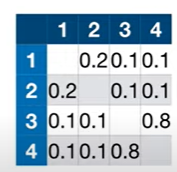
\includegraphics[scale=1]{proximitymatrix.png}
     \end{center}
  \begin{enumerate}
      \item  To estimate the missing data in original data set , we initially assume the missing data as the majority in classification and average in regression. 
 \item Later , we run the data through all the decision trees and create a proximity matrix with probabilities that both the values end at the same leaf node.

  \item  we calculate the weighted frequencies($WF$) given by equation \eqref{eq:1.1} for classification , and equation \eqref{eq:1.2} for regression;Where $f$ is the frequency of the value, and $w$ is the weight. these substitute the missing data.
  \item we iterate the process a few times , so get the most accurate value,similar iterative methods are used for new data also.
    \end{enumerate}
  \begin{align}
      WF_c=f_ow_o +f_1w_1 \label{eq:1.1} \\
      WF_R=\sum_{i=1}^n f_iw_i \label{eq:1.2}
  \end{align}
  
  Thus, random forest can be used when we have a lot of features and it's stability due to majority voting is it's selling point.
  
\end{document}